\chapter{Background \& Theory} \label{chap_theory}

\section{Overview}

This chapter presents the background theory for information flow security and security typing mechanisms, with reference to the supporting literature. Specifically, it provides context for the model of Mandatory Access Control, the theory for which underpins most security typing implementations, as well as for the widely used Java security model. Information flow security, and its expression through the notion of \textit{non-interference} are explained along with key concepts around the declassification of information. Finally, security typing itself is introduced, as are the policy models for security typing from the literature.

\newpage

\section{Security Context}

Information security in practice revolves around three key goals colloquially known as the `CIA Triad' \cite{krutz2010cloudsec}:

\begin{itemize}
	\item Ensuring information is appropriately \textit{Confidential} (the focus of this thesis)

	\begin{itemize}
		\item Example: a secret password being leaked is a confidentiality violation
	\end{itemize}
	
	\item Ensuring information has \textit{Integrity}
	
	\begin{itemize}
		\item Example: a database being accessed and records falsified is an integrity violation
	\end{itemize}
	
	\item Ensuring information is \textit{Available}
	
	\begin{itemize}
		\item Example: a Denial of Service (DoS) attack causing a website to crash is an availability violation
	\end{itemize}

\end{itemize}

Most language-based security features focus on the confidentiality and integrity of information; that is, ensuring that secret information remains secret, and that information which needs to be trusted is in fact trustworthy.

Here, systems which aim to ensure confidentiality are examined, though similar mechanisms may also be used to control integrity.

\section{Access Control}

The most common mechanism used in computer systems to ensure confidentiality is \textit{access control}: associating some `permissions' with users of a system and restricting the actions they are able to perform based on these permissions. The principles of limiting user access is most frequently applied through one of two approaches: \textit{Discretionary} Access Control, and \textit{Mandatory} Access Control

\subsection{Discretionary Access Control} \label{theory_dac_def}

Discretionary Access Control (DAC) is the basis of most operating system-level permissions systems, including those in Unix-like operating systems \cite{sandhu1996role}, and those implemented in modern versions of Windows.

Central to DAC is the \textit{Access Matrix} \cite{sandhu1994access} -- a two-dimensional matrix indexed by \textit{subjects} (users or groups) and by \textit{objects} (documents, files or other information to be accessed). The values in the matrix determine whether a given subject has permissions to access a particular object, and this is enforced with a run-time check: when the user attempts to access an object they lack permissions for, they will see a message indicating the check's failure.

With any non-trivial set of users and documents, the size of the Access Matrix will be prohibitively large, and so most commonly the Access Matrix is implemented using Access Control Lists (ACLs), which are equivalent to columns of the Access Matrix. An ACL is stored alongside every object, indicating which subjects may access it \cite{sandhu1994access}.

\subsection{Limitations of Discretionary Access Control} \label{theory_dac_limitations}

Access control mechanisms attempt to control confidentiality by inserting checks at boundary points where information flows between subjects.

Consider, a scenario in which a user Alice has a diary, which she wishes to keep secret. Alice allows Betty to read her diary, but does not wish to allow a third user, Mal, to read it. Using DAC, an Access Control List for the diary would list Alice and Betty, but not Mal. Then, if Mal attempts to read the diary the access check will fail, preserving confidentiality.

\begin{figure}[h!]
	\centering
	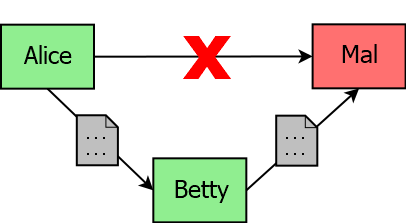
\includegraphics[scale=0.5]{content/lit_theory/access_control_example.png}
	\caption{Circumventing an Access Control Check}
	\label{fig:theory_access_control_failure}
\end{figure}

However, suppose Betty now attempts to read Alice's diary. The access check allows this, since it is within policy. Betty reads the diary and makes a copy of it, which she then transmits to Mal, as shown in \autoref{fig:theory_access_control_failure}. Since Betty's copy may have whatever policy she desires, the existing access policy on the diary does not prevent Mal from reading the copy.

The root cause of this failure is that the access control policy merely performs boundary checks, but does not model the \textit{propagation} of information once those checks have been passed.

\subsection{Mandatory Access Control} \label{accesscontrol_mac}

Mandatory Access Control (MAC) systems are most commonly associated with the military, and are generally used in situations where confidentiality is of primary importance. In a MAC system, all data has a \textit{classification}, and users operate with a \textit{clearance} \cite{sandhu1994access}. 

In the simplest case, the set of classifications is just an ordered list -- for instance, `Unclassified' $ < $ `Classified' $ < $ `Secret' $ < $ `Top Secret' (represented in \autoref{fig:theory_lattice_diagrams} (a)). A user with `Secret' clearance, then, cannot access or modify `Top Secret' documents.

More flexible access control policies may be implemented under the Bell-LaPadula lattice model \cite{bell1973lattice}, which is at the heart of most modern MAC systems. Under this model, classifications form a \textit{lattice} -- a set partially ordered by a flow relation (written $ \succeq $) where, for every possible pair of elements, a `least upper bound' (or `join', written $ \sqcup $) and `greatest lower bound' (or `meet', written $ \sqcap $) may be found.

\begin{figure}[h!]
	\centering
	\begin{subfigure}[t]{0.2\textwidth}
		\begin{tikzpicture}
		\node[dot, label=left:$ TS $] (TS) at (0, 3) {};
		\node[dot, label=left:$ S $] (S) at (0, 2) {};
		\node[dot, label=left:$ C $] (C) at (0, 1) {};
		\node[dot, label=left:$ U $] (U) at (0, 0) {};
		
		\draw[edge] (S) to node[right, sloped, anchor=north] {$ \preceq $} (TS);
		\draw[edge] (C) to node[right, sloped, anchor=north] {$ \preceq $} (S);
		\draw[edge] (U) to node[right, sloped, anchor=north] {$ \preceq $} (C);
		\end{tikzpicture}
		\caption{}
	\end{subfigure}
	~
	\begin{subfigure}[t]{0.1\textwidth}
		\begin{tikzpicture}
		\node[dot, label=above:$ A \sqcup B $] (AuB) at (0, 2) {};
		\node[dot, label=left:$ A $] (A) at (-1, 1) {};
		\node[dot, label=right:$ B $] (B) at (1, 1) {};
		\node[dot, label=below:$ A \sqcap B $] (AnB) at (0, 0) {};
		
		\draw[edge] (AnB) to node[right, sloped, anchor=north] {$ \succeq $} (A);
		\draw[edge] (AnB) to node[right, sloped, anchor=north] {$ \preceq $}  (B);
		\draw[edge] (A) to node[right, sloped, anchor=south] {$ \preceq $} (AuB);
		\draw[edge] (B) to node[right, sloped, anchor=south] {$ \succeq $} (AuB);
		\end{tikzpicture}
		\caption{}
	\end{subfigure}
	\caption{Example Bell-LaPadula Model Lattices}
	\label{fig:theory_lattice_diagrams}
\end{figure}



In the MAC context, for policies in a lattice structure a user at clearance $ A $ can access information at classification $ B $ if $ A \succeq B $ (which may be read as ``$ B $ is less restrictive than $ A $"). Given any two classifications $ A $ and $ B $, one can find the least restrictive classification which enforces both, $ A \sqcup B $, and the most restrictive classification which users at either clearance $ A $ or $ B $ can read, $ A \sqcap B $.

The Bell-LaPadula model may be applied to an access control problem concerning users (or `subjects') and classified documents (or `objects') via two rules \cite{sandhu1993lattice}:

\begin{description}
	\item[Simple Security Property -- `No Read Up'] A subject with clearance $ C_s $ may access an object with classification $ C_o $ if and only if $ C_s \succeq C_o $
	
	\item[* Property -- `No Write Down'] A subject with clearance $ C_s $ may only modify an object with classification $ C_o $ if $ C_o \succeq C_s $
\end{description}

The Simple Security Property prevents users with insufficient clearance from accessing highly classified data. But the * Property is also important: it states that a user with high clearance cannot modify data at a low classification. For the scenario presented in \ref{theory_dac_limitations}, this would prevent Betty from creating a copy of the document and sending it to Mal, as Betty may not copy the document to a lower classification. In effect, this introduces a control on the \textit{propagation} of that information.

Lattice-based Mandatory Access Control may be applied to computer systems, just as Alice's diary or to physical documents. Such systems generally use a `high water mark' approach \cite{jones1975highwatermark}, allowing programs to begin at low clearance and only moving to higher clearance as needed.

\section{The Java Security Model} \label{theory_javasec}

The Java programming language was designed in the context of emerging internet technologies, with the explict use case of users downloading and running `applets' from web pages \cite{gong1999javasecspec}. As such, security was a core consideration in Java's design -- the original design goals document \cite{javadesignprinciples} specifies that ``applications written in the Java programming language are secure from intrusion by unauthorized code."
 
Java is type safe and memory safe, which reduces the possibility of programmer error leading to exploitable flaws in an application. Java's application sandbox takes a three-pronged approach to security in the context of applets which may be downloaded from a remote server, having a Bytecode Verifier, the Class Loader, and the Security Manager \cite{mcgraw1999securingjava}.

The Bytecode Verifier and the Class Loader concern the loading of new classes into a running Java Virtual Machine (JVM). The Bytecode Verifier analyses the class to ensure it maintains the class format, does not perform illegal casts, and that it obeys Java's typing rules more generally (e.g. that private methods may not be accessed outside of a class, final methods may not be overridden) \cite{lindholm2014java}. The Class Loader performs the actual loading of a class into the JVM; the `primordial' Class Loader \cite{mcgraw1999securingjava} loads the Java API classes, and other classes may be loaded by a user-specified \mono{ClassLoader} instance.

\subsection{The Security Manager \& Stack Inspection}

The final element of the sandbox model is the \mono{SecurityManager} class. When enabled, an instance of \mono{SecurityManager} runs in the JVM, and performs runtime access control: when a potentially sensitive action is undertaken, the Security Manager checks the permissions of the calling class based on a system policy, usually specified by an external policy file. This represents a \textit{discretionary} access control model as per the definition in \ref{theory_dac_def}. If the permission check fails, a \mono{SecurityException} is thrown \cite{gosling2014java}. A check is typically of the form \cite{javasecmanagerdoc}:

\begin{minted}{java}

SecurityManager sm = System.getSecurityManager();
Object context = sm == null ? null : sm.getSecurityContext();
if (sm != null)
	sm.checkPermission(new FilePermission("someFile.txt", "read"), context);
\end{minted}

Permission checks are performed using stack inspection \cite{gong2003javasecurity}: every frame on the call stack below the sensitive operation is examined, and if \textit{any} frame does not have the required permissions, the check fails. Java provides the \mono{doPrivileged} construct to bypass full stack inspection \cite{gong2003javasecurity} where this functionality is desired.

\section{Information Flow Security}

Access control mechanisms limit the \textit{permissions} of a subject attempting to access data. Many programs and operating systems make use of Discretionary Access Control. Such access-check based mechanisms do not restrict the way in which information \textit{propagates}, which leads to circumvention as described in \ref{theory_dac_limitations}.

The Bell-LaPadula Lattice Model used in MAC may be used to control the \textit{flow} of information rather than merely check for access. The *-property as presented in \ref{accesscontrol_mac} provides a primitive form of this: it prevents even those with high clearance from `leaking' high classification data to a low level, thereby controlling its flow rather than simply performing an access check.

\section{Formal Non-interference \& Static Information Flow} \label{theory_if_noninterference}

The traditional MAC model, including controls against information leaks (such as via the *-property), may be implemented in a real system via runtime-enforced access control checks. However, an important question remains: how does the program's author know whether it is implemented \textit{correctly}? Many security issues are the result of unintentional programmer error, and so it is useful to approach Information Flow security from the perspective of program verification.

This goal can be more clearly defined through the notion of `non-interference'. A program is said to be non-interfering if, given any two program executions which are identical in terms of their low confidentiality input, the results and behaviour of the executions are indistinguishable in terms of their low confidentiality output \cite{sabelfeld2003if}. Equivalently, a program is non-interfering if there is no \textit{dependency} of low confidentiality data on high confidentiality data \cite{cohen1977declassification}.

For example, consider a function $ f: L \times H \rightarrow L \times H $, where $ L $ is the set of integers at low confidentiality and $ H $ is the set of integers at high confidentiality, such that $ f(l, h) = \langle \frac{l + h}{2}, \frac{l + h}{2} \rangle $. Then $ f $ is a function that returns the average of its low and high inputs in both its low and high outputs. This function is interfering: the value of the low output depends on the value of the high input.

Consider instead $ g: L \times H \rightarrow L \times H $, where $ g(l, h) = \langle l + 5, \frac{l + h}{2} \rangle $; $ g $'s high output is the same as that of $ f $, but its low output simply adds $ 5 $ to the low input $ l $. This function is \textit{non-interfering}: the low output has no dependency upon the high input.

For programs written in languages like Java which allow mutable state, it is difficult to accurately capture a program's entire output as a function of its input. Instead, non-interference checking for these languages considers the flow of information through the system, through assignment to variables and through calls to method which incur side effects (such as printing the value of a variable to the screen, or to a file). So, for instance, the following code would be invalid:

\begin{algorithmic}
\State $ high := 1 $
\State $ low := high $
\end{algorithmic}

Clearly, assigning the value of a high confidentiality variable to a variable with low confidentiality violates the policy, and in a non-interference sense allows an attacker with low confidentiality privileges to learn the high confidentiality value.

\subsection{Implicit Flows}

\citeauthor{denning1977certification} \cite{denning1977certification} categorise the flows of information within a program into \textit{explicit} and \textit{implicit} flows. An explicit flow $ x \rightarrow y $ is one such as an assignment $ y := x $, where the value assigned to a variable $ y $ is directly dependent on the value of variable $ x $. An implicit flow $ x \rightarrow y $ is then any arbitrary flow $ z \rightarrow y $ where $ z $ may not be directly related to $ x $, but whether or not the statement is executed depends on the value of $ x $.

A simple example of an implicit flow causing an information leak is one where execution branches based on the value of a high confidentiality variable:

\begin{algorithmic}
	\State $ high := 0 $
	\State $ low := 0 $
	\If {$ high = 5 $}
		\State $ low := 1 $
	\Else
		\State $ low := 0 $
	\EndIf
\end{algorithmic}

Here, someone with access to the $ low $ variable knows that $ low $ will only have the value $ 1 $ if $ high $ has the value $ 5 $. After this code executes, they can see that $ low = 0 $, and therefore $ high \ne 5 $. They do not know the actual value of $ high $ but they have still learned some information about it.

For a program to be non-interfering, a passive attacker must not be able to distinguish \textit{any} information about high confidentiality data; hence implicit flows which allow an attacker to learn high confidentiality information must be prevented \cite{sabelfeld2003if}.

To handle implicit flow of confidentiality via the flow of control, the confidentiality of the execution \textit{context} must be considered. The above snippet's conditional statement represents a `high context' where assignments to low confidentiality variables is impermissible.

\subsection{Covert Channels \& Attacker Model}

Consider the following program:

\begin{algorithmic}
	\State $ low := 0 $
	\If {$ high = 5 $}
		\For{$ i := 1 $ \textbf{to} $ 1000000000 $}
			\State skip
		\EndFor
	\Else
		\State skip
	\EndIf
\end{algorithmic}

By the conventional definitions of information flow, considering both explicit and implicit flows, this program is non-interfering: the value of $ low $ does not in any way depend on the value of $ high $. Yet, someone observing this programs output would be able to learn information about the value of $ high $: the program will clearly take significantly longer to execute in the case where $ high = 5 $.

A program can only be considered secure \textit{with respect to its environment} \cite{sabelfeld2003if}, and the standard construction of non-interference does not consider the timing of a program as a channel for the transmission of information; hence, this kind of information leak is considered a `covert channel' leak.

\citeauthor{sabelfeld2003if} \cite{sabelfeld2003if} address a number of possible covert channels which impact on information flow analysis, including timing channels like the above, termination-sensitivity (i.e. whether a program terminates at all), system power usage, and probabilistic channels for programs with stochastic behaviour. Notions of non-interference which examine these channels may be constructed, though doing so will further restrict the potential acceptable programs which may be written.

Hence, proving a program's non-interference under the model presented thus far is not a panacea: a program's environment and attacker model must still be considered. In some contexts, `timing-sensitive' non-interference may be necessary, but enforcing that a program will never differ in execution time based on high confidentiality information has quite obvious drawbacks in the performance of a valid program and in the kinds of programs which may be written.

\section{Enforcement \& Security Typing}

\subsection{Enforcement Mechanisms}

Enforcement of access control mechanisms is typically done at runtime, as with the Java security model (described in \ref{theory_javasec}), by performing checks whenever a potentially sensitive operation is performed. While some implementations of information flow security are also based on runtime checks \cite{austin2009runtimeflow} \cite{degroef2012flowfox} \cite{polikarpova2016lifty}, treating information flow as a problem of program verification allows for a guarantee of non-interference with no runtime overhead.

\subsection{Security Typing}

In \citetitle{denning1977certification}, \citeauthor{denning1977certification} \cite{denning1977certification} provide a mechanism to verify a program as correctly respecting a lattice-model policy using type checking. All variables are assigned a classification, and the analyser ensures that the policy is not broken under any execution path via a set of type semantics. A language which makes use of type checking-based flow verification is considered a \textit{security typed} language.

The nature of the type semantics used, and hence the complexity of the typing ruleset, depends on the policy model being enforced. \citeauthor{denning1977certification} \cite{denning1977certification} enforce a Bell-LaPadula lattice model policy, and so variable assignments from a variable with a lower security type to a higher security type would fail to compile, as would modification of low confidentiality variables inside a high conditional.

\subsection{Undecidability in the General Case}

The type checking approach to proving non-interference is necessarily conservative: there will always be some programs which are non-interfering which will nonetheless be rejected by the static analysis. This goes beyond being a limitation of current models: determining a condition which is both necessary and sufficient for a program to be non-interfering is an undecidable problem \cite{denning1977certification} \cite{landi1992undecidability} -- it may be reduced to the halting problem \cite{sabelfeld2003if}.

In practice, systems for statically analysing information flow attempt to ensure that they reject as few \textit{useful} valid programs as is feasible.

\section{Declassification}

A program which is provably non-interfering provides useful guarantees about a program's behaviour: in the military context for which MAC was designed, it ensures that a program running in a high confidentiality environment cannot declassify information to a lower level. However, in most contexts, requiring strict non-interference prevents useful and necessary programs from being written.

One example of this is a `password checker' program. The true value of the password is confidential, and the user must provide a correct guess in order to log in. Clearly the operation of the program depends on the value of the high confidentiality password, and a user attempting to log in learns some information about it -- even if rejected, the user has learned that the true password is \textit{not} equal to their guess.

A password checker is interfering by design: it has to give feedback on whether the user's guess matches the true password. But this does not violate the desired security properties, since the search space for possible passwords is large, and the user may only guess one at a time.

Rejecting \textit{all} interfering programs makes it very difficult to write even simple programs like a password checker. Hence, security typed languages provide `declassification' mechanisms to allow interference, but only when a programmer explicitly declares it.

\subsection{Dimensions of Declassification}

Mechanisms for declassification may be categorised by the controls they aim to implement. \citeauthor{sabelfeld2005dimensions} \cite{sabelfeld2005dimensions} provide four `dimensions' of declassification: \textit{what}, \textit{who}, \textit{where} and \textit{when}.

A `selective' declassification mechanism controls \textit{what} information or \textit{how much} information may be released. An `ownership-based' declassification mechanism regulates \textit{who} may release information; this is generally accompanied by a policy model which encodes ownership, such as the Decentralised Label Model discussed in \ref{theory_if_dlm}. Models of `intransitive non-interference' \cite{roscoe1999intransitive} place controls on \textit{where} information may be declassified, requiring that information only be released through some form of sanitising function. Finally, mechanisms may control \textit{when} information may be released -- whether relative to other events in the program, or in absolute terms.

\section{Policy Models for Security Typing}

\subsection{The Denning Lattice Model}

Modern implementations of security typing derive primarily from the model proposed by \citeauthor{denning1977certification} \cite{denning1977certification}, previously discussed in \ref{theory_if_noninterference}. This model assumes that classifications are determined by a central authority; in a security typing implementation, this is the programmer. The lattice model makes it possible to implement both simplistic `totally ordered' policies and policies with more complex lattice structures. It also allows for the combination of existing policies within the lattice using the join and meet operators.

\subsubsection{Selective Declassification Mechanisms}

A simple approach to declassification within a standard lattice model is to include a `declassify' syntax, wherein the classification of a variable may be changed to one of lower confidentiality \cite{denning1974declassification}. This allows for any interfering program to be written (and hence allows the programmer to break the guarantees that the type system would provide), but it requires them to explicitly declare what information they  wish to declassify.

\citeauthor{volpano2000declassification} \cite{volpano2000declassification} propose a declassification construct which guarantees information may only flow against the stated policy in worse-than-polynomial runtime complexity. Using this mechanism, the password checker example would be valid, since finding the actual value of the password requires an exponential time brute force checking of all possibilities. Being more restrictive, this approach is more difficult to apply to real world programs.

\subsection{The Decentralised Label Model} \label{theory_if_dlm}

The Decentralised Label Model (DLM) proposed by \citeauthor{myers1997if} \cite{myers1997if} extends the Bell-LaPadula lattice model by removing the need for a central authority which determines all classifications.

Instead, under the DLM subjects (or `principals') within the system may define their own policies on data, specifying which other subjects \textit{they believe} the data should be able to flow to. These policies still form a lattice, and so the type checker enforces the join of all subjects' policies on the data. This can be used to model `ownership' of data, and even systems where subjects do not trust each other to respect confidentiality.

The DLM is discussed in more depth in Chapter \ref{chap_jif_para} as it is the policy framework used by the JIF programming language.

\subsubsection{Selective Declassification Mechanism}

As with Denning model systems, `declassify' syntax may be used with the DLM to provide a control for \textit{what} information may be released. However, the DLM also allows for controls on \textit{who} may declassify information: a given subject may only declassify policies under their own authority, and so cannot reduce the confidentiality of data which does not `belong' to them.

\subsection{Flow Lock Policy Definition}

The Denning model uses MAC classification labels, and the DLM extends this with a decentralised model of information ownership. Both models control declassification with the introduction of explicit constructs which declare that information downgrade is taking place. \citeauthor{broberg2006flow} \cite{broberg2006flow} propose an alternative form of policy specification using predicate logic.

Under this model, policies are statements of which subjects may access the data. Policies may specify individual subjects (e.g. a policy stating ``Alice may read this information"), or may universally quantify over subjects belonging to some class (e.g. ``All subjects who are System Administrators may access this information").

This model is discussed in more depth in Chapter \ref{chap_jif_para} as it forms the basis of policy definition in the Paragon programming language \cite{broberg2013paragon}.

\subsubsection{Dynamic Policy}

This model's eponymous `Flow Lock' system allows it to represent dynamic flow policy -- that is, policy which cannot be represented in a static lattice structure. This presents an alternate approach the declassification problem:  policy based on ``what" information is declassified (as modelled in the Denning model or in the DLM) is viewed as a special case of dynamic policy, as are other models based on ``when" or ``where" declassification occurs.

A Flow Lock is a runtime boolean value that may be in either an `open' or `closed' state. The lock may then guard a flow policy, allowing for policies of the form ``Alice may read this information \textit{if} the lock \mono{IsUnlocked} is open". Although locks are runtime values, their values throughout the program are still approximated statically through the type checker. Since locks may change state at runtime, they can be used to not only control \textit{what} information is declassified, but also \textit{when} information is declassified; such time-variant policies cannot be easily encoded in the DLM or in Denning model security type systems.

The Flow Lock concept was extended further in a second paper \cite{broberg2010paralocks} to include \textit{parametrised} locks, called `Paralocks'. Parametrised locks allow for policies such as ``Alice may read this information if the lock \mono{IsUnlocked}(Alice) is open".

Unary (single argument) locks can then easily represent policies with dynamic \textit{roles}, like ``Any employee may access this information if they are currently a manager", built using a quantification over employees and an \mono{IsManager(Employee)} lock. Binary locks, on the other hand, can represent relationships between subjects.

The semantics of Paralocks provide a generalisation of existing policy mechanisms: it is possible to encode the DLM, and hence any policy the DLM can encode, using Paralocks \cite{broberg2010paralocks}.
%\subsection{Selective Declassification}
%
%Selective declassification mechanisms provide an `escape hatch' from the security typing system. Through these mechanisms, information may flow in a way which contravenes the Information Flow policy. As such, these mechanisms must be tightly controlled.
%
%
%
%\citeauthor{sabelfeld2004model} \cite{sabelfeld2004model} propose `delimited release' -- a selective declassification mechanism which allows for more control over the semantics of \textit{what} is supposed to be released during a declassification. If the actual statement declassifies more information than was defined, then the program is rejected by the type checker.
%
%Another such mechanism, proposed by \citeauthor{myers1997if} \cite{myers1997if}, provides a safer form of the declassify operator, relying on a more complex decentralised policy model (discussed in more depth in \ref{if_static_models}), which gives policies an \textit{owner}. Declassification can then only be performed under the authority of the owner of a policy.
%
%
%
%FLOW LOCKS / PARALOCKS

%\section{Enforcement}
%
%\subsection{Statically Enforced Models} \label{if_static_models}
%
%DENNING
%
%DLM
%
%PARAGON
%
%\subsection{Runtime Enforced Models}




%\section{The Decentralised Label Model}
%
%\section{Logic-Based Policies \& The Paralock Model}
%
%\section{Other Models}


%** MOVED FROM COMPARISON... **
%
%The `JFlow' language, through both the paper \cite{myers1999jflow} that proposed it and its subsequent implementation as Java Information Flow (JIF), has become the dominant language and the dominant paradigm in security typing and static information flow control languages more generally.
%
%As articulated by \citeauthor{broberg2013paragon} in \citetitle{broberg2013paragon} \cite{broberg2013paragon}, JIF may be regarded as a `second-generation Information Flow language'. Its Decentralised Label Model allowed for more flexible and more useful policies to be expressed than the straight Mandatory Access Control lattice that had been at the centre of most prior work, and its implementation as an extension of the popular Java language made it comparatively practical to work with.
%
%Under this taxonomy, Paragon is then a `third-generation Information Flow language'. It discards lattice-based policy definition entirely in favour of policies which may defined through logical expressions. This abstraction, combined with the Paralock construct which allows for policies which model relations and which vary over the lifetime of a running program, broadens the scope of what security requirements can be expressed.
%
%The Paralock construct which Paragon introduces allow for policies which vary over the lifetime of a running program, something which cannot be represented effectively under JIF's policy model. In addition, Paralocks can model relations between actors of arity zero, one or two, and through the use of binary relations, the Decentralised Label Model can in fact be written within Paragon's policy language. That is, JIF's policy mechanism can be encoded using Paragon's.